\documentclass[../main.tex]{subfiles}
\begin{document}

\chapter{Lecture 24 - 09-06-2020}
\section{Neural Networks}

\subsection{Feedforward NN}
$$
f : \barra{R}^d \rightarrow \barra{R}^n
$$
Done with a combination of preditors.
$$
g(x) = \sigma(w^T \, x) \qquad \textbf{$\sigma$ is  a nonòinear activation function}
$$
Entire structure is a DAG:
$$
G= (V,E) \quad DAG \textit{  directed and acyclic graph}
$$
\begin{figure}[h]
    \centering
    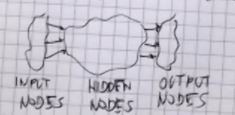
\includegraphics[width=0.3\linewidth]{../img/lez24-img1.JPG}
    \caption{}
    %\label{fig:}
\end{figure}\\
Multilayer NN (special case of Feedforward)
\begin{figure}[h]
    \centering
    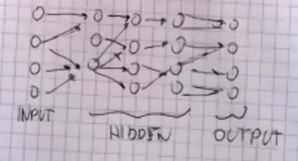
\includegraphics[width=0.3\linewidth]{../img/lez24-img2.JPG}
    \caption{}
    %\label{fig:}
\end{figure}\\
Computing a function:
$$ g(\cdot) = \sigma(w^T \cdot)$$
where $\cdot$ is the input of the previous layer.
\\ 
We are going to split the nodes:
$$
V = V_m \cup V_{hid} \cup V_{out} \qquad |V_{in}| = d
$$
If $(i,j)$ is an edge:
$$
(i,j) \in E \Rightarrow w_{ij} \in \barra{R} \qquad \textit{ where $i$ and $j$ are nodes}
$$
$W$ weighted matrix:
$$
w_{ij}= 0 \quad if \quad (i,j) \not \in E
$$
We have then $G,w, \sigma$ parameters that define a function compute by the network:
$$
f_{G,w,\sigma} : \barra{R}^d \rightarrow \barra{R}^n
$$
Let's pick any node $j$ that $ j \in V \setminus V_{in}$:
$$
w(j) : \{ w_{ij} : (i,j)
$$
\begin{figure}[h]
    \centering
    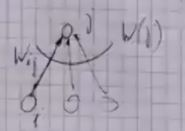
\includegraphics[width=0.3\linewidth]{../img/lez24-img3.JPG}
    \caption{}
    %\label{fig:}
\end{figure}\\
MANCAAAA
\\\\
Each node $j$ has a state value which is evaluated during the computation of the function.
$$
V_j = \sigma(w(j)^T v(j))
$$
\begin{figure}[h]
    \centering
    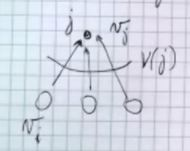
\includegraphics[width=0.3\linewidth]{../img/lez24-img4.JPG}
    \caption{}
    %\label{fig:}
\end{figure}\\
\begin{figure}[h]
    \centering
    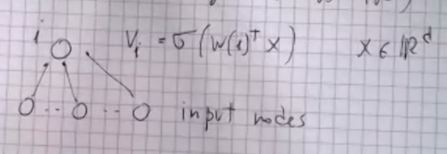
\includegraphics[width=0.3\linewidth]{../img/lez24-img5.JPG}
    \caption{}
    %\label{fig:}
\end{figure}\\
\newpage
$$
V_i = \sigma(w(i)^T x) \qquad x \in \barra{R}^d
$$
$$
f_{G,w,\sigma}(x) \qquad v_i = \sigma(w(j)^T v(j))
$$
\begin{figure}[h]
    \centering
    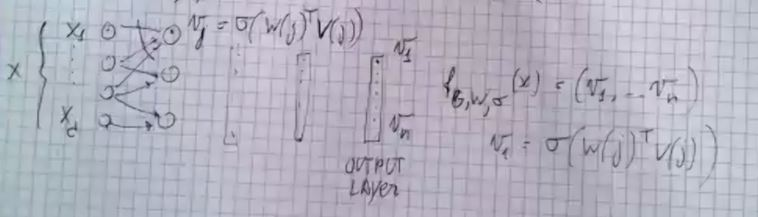
\includegraphics[width=0.5\linewidth]{../img/lez24-img6.JPG}
    \caption{}
    %\label{fig:}
\end{figure}\\
$$
f_{G,w,\sigma} (x) = (v_1,...,v_n) \qquad v1= \sigma (w(j)^T v(j))
$$
What are the parameters I learn?\\
$G, \sigma$ fixed and $w$ is trained.
\\
I can define a class $F$:
$$
F_{G,\sigma} \textbf{class of all predictors $f_{G,w,\sigma}$ for $w$ variable}
$$
$\sigma$ is the identity and we can do other model like linear regression etc.
\begin{figure}[h]
    \centering
    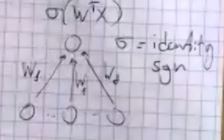
\includegraphics[width=0.3\linewidth]{../img/lez24-img8.JPG}
    \caption{}
    %\label{fig:}
\end{figure}\\
\newpage
\bred{Case of single output node:}
\begin{figure}[h]
    \centering
    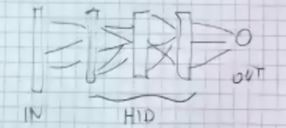
\includegraphics[width=0.3\linewidth]{../img/lez24-img9.JPG}
    \caption{}
    %\label{fig:}
\end{figure}\\
In classification:
$$
v_0 = f_{G,w,\sigma}(x) = sgn (w(0)^T v(0))
$$
In regression:
$$
w(0)^T v(0)
$$
This depends on the problem. How do I choose the activation function $\sigma$?
Could be a Sigmoid or Relu (0 in negative and 1 positive part) or other variant of this like Leaky Relu. \\
The first one is bounded the other one are not.
\begin{figure}[h]
    \centering
    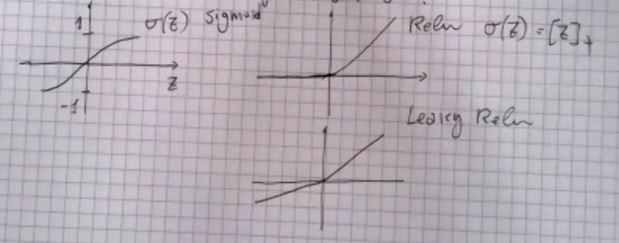
\includegraphics[width=0.5\linewidth]{../img/lez24-img10.JPG}
    \caption{}
    %\label{fig:}
\end{figure}\\
How many layers? 
\\ How many nodes in each layer?
\\ Patter connectivity between layers?
\\ Activation function?
\\
In order to define our class $F_{G,\sigma}$:
we are gonna ask ourself some structural question. How many layers do I need in general? Is there a minimum range of layers?
\newpage

\bred{Theorem}
$$
\forall \ d \ \exists \ G = (V,E) \textit{\ with $d+1$ input nodes, one hidden layer, one output node }
$$
$$ s.t \ F_{G,sgn} \textit{ contains all function of the form} f:\{-1,1\}^d \rightarrow \{-1,1\}
$$

\bred{Proof}
\begin{figure}[h]
    \centering
    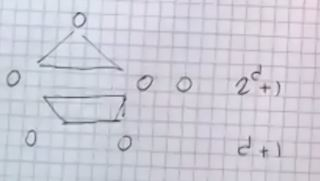
\includegraphics[width=0.5\linewidth]{../img/lez24-img11.JPG}
    \caption{}
    %\label{fig:}
\end{figure}\\
$$
f: \{-1,1\}^d \rightarrow \{-1,1\}
$$
$$
\bar{x}_1,...,\bar{x}_N \qquad f(\bar{x}_i) = 1 \qquad N \leq 2^d
$$
The $i$-$th$ hidden node computes the function: $$g_i(x) = sgn(\bar{x}^T \bar{x}_i - d +1) \qquad \bar{x} \rightsquigarrow \hat{x}(\bar{x},1) 
$$
$$
w(i) = (\bar{x}_i, -d+1) \qquad 
w(i)^T \hat{x} = \bar{x}^T \bar{x}_i -d +1
$$
\begin{figure}[h]
    \centering
    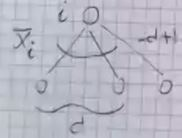
\includegraphics[width=0.3\linewidth]{../img/lez24-img12.JPG}
    \caption{}
    %\label{fig:}
\end{figure}\\
$$
x^T x_i = \begin{cases}
d \qquad \qquad \ \ if \ x=x_i
\\
\leq d-2 \qquad if \ x \neq x_i
\end{cases}
$$

\newpage
Let's see the output layer
$$
f(x) = g_1(x) \vee ... \vee g_N(x)
$$
\begin{figure}[h]
    \centering
    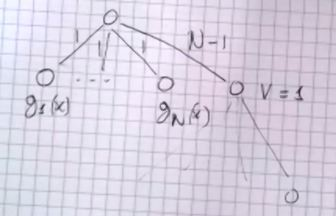
\includegraphics[width=0.4\linewidth]{../img/lez24-img13.JPG}
    \caption{}
    %\label{fig:}
\end{figure}\\
The function compute by the output node is :
$$
sgn(w(0)^T v(0)) = \sum_{i=1}^N g_i(x) w_{i,0}  + N -1
$$
where $\sum_{i=1}^N g_i(x) w_{i,0}$ is equal to $-N +1$ to obtain $1$.
$$
x \ s.t \ f(x) = -1 \qquad g(x) = -1 \qquad i = 1,...,N
$$
$$
x \ s.t. \ f(x) = 1 \qquad \exists i : g_i(x) = 1
$$\\
I can definetely use more than one layer since exponential is not good. Maybe you can use fewer node, still potentially able to generate a classifier.
\\\\
\bred{Theorem}\\
$
\forall d \in \barra{N}
$ let $s(d)$ be the smaller integer \\ s.t. $\exists \ G = (V,E)$ with $|V| = s(d)$ \\ s.t. $F_{G,sgn}$ contains all functions $f: \{-1,1\}^d \rightarrow \{-1,1\}$ then $|V|= \Omega (2^{\frac{d}{3}})$
\\
If inputs are not binary we will use a sigmoid function. So 1 hidden layer is enought to approximate all function of the form:
$$
f: [-1,1]^d \rightarrow [-1,1]
$$
If you want to learn everything you need an exponential number of nodes.

\newpage
\section{Deep Learning}
I have many hidden layers, not too many nodes in each layer. 
\\
I am choosing $G$ with a specific profile (tall and skinny network).

$$
F_{G_{dept},\sigma} \quad compared \ with \quad F_{G_{fat},\sigma}
$$
\begin{figure}[h]
    \centering
    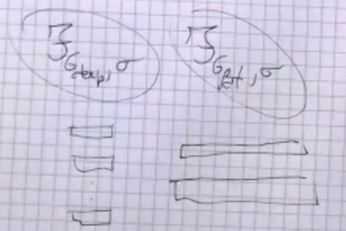
\includegraphics[width=0.4\linewidth]{../img/lez24-img14.JPG}
    \caption{}
    %\label{fig:}
\end{figure}\\
Usually, the first one should be the better one. \\
$$ |V'| > |V|  \qquad 
G \rightarrow G' \qquad F_{G,\sigma}
$$
Either increase size of 2 layer or add more layers:
$$
|F_{G', \sigma}| \gg |F_{G", \sigma}|
$$
where $G'$ are new layers and $G"$ are the fatter layers.
\newpage
\subsection{Convolution Neural Network}
\begin{figure}[h]
    \centering
    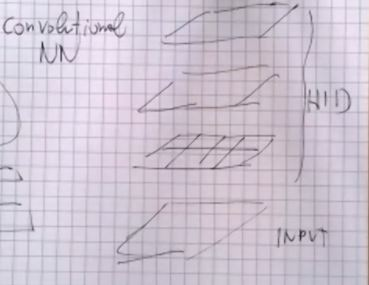
\includegraphics[width=0.4\linewidth]{../img/lez24-img15.JPG}
    \caption{}
    %\label{fig:}
\end{figure}
== MANCAAAA FOTO GiUSTA ====
\\\\
Using convolutional NN.
We will recognise some shape (like presence of angles or simple geometric form obtained by combine the edge detector in the previous layers.
If you have several layers you can have more more specific shapes combine the previous simpler layers.
\\\\
\subsection{General infos about Neural Networks}
NN are trained using stochastic gradient descent.
$$
W \qquad w_{ij} \leftarrow w_{ij} - \eta_t \frac{\eth \ell_{z_t}(w)}{\eth w_{ij}} 
$$
$Z_t$ is randomly drawn from training set.
\\
$$
\ell_t(w) = \ell(f_{G,w,\sigma}(x_t),y_t) \quad \forall (i,j) \in E
$$
We have $ \nabla \ell_t(w)$
\\ The gradient component $\frac{\eth \ell_{z_t}(w)}{\eth w_{ij}} \quad (i,j) \in \sqrt[]{s}$ is computed using a technique called "error backpropagation"
\\
$\ell_t(w)$ is not convex!
\begin{figure}[h]
    \centering
    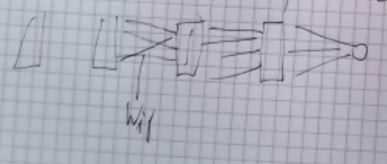
\includegraphics[width=0.4\linewidth]{../img/lez24-img16.JPG}
    \caption{}
    %\label{fig:}
\end{figure}
Gradient descent will not terminate in: $$
w^* = arg \min_w \hat{\ell}_s (w)
$$
\\
\bred{AutoML to determine hyperparameter!}
\end{document}